\setcounter{section}{0}
\section{Health and Well Being}
Health is one of the most important, if not the most important aspects of a person's life. For this reason, over the years, different organisations have established different guidelines on how to stay healthy, thus increasing people's life expectancy and quality of life. Among these, the most widely worldwide recognized is the World Health Organization (WHO) \cite{Who} that provides several guidelines not only in term of physical activity, covering also other health aspects. \newline As far as concerns the physical activity, the WHO estimates that 1 in 3 adults and 4 in 5 adolescents do not do enough physical activity, with adolescents girls less active than adolescents boys and with inactivity levels that increases after 60 years of age. This level is expected to rise due to country economic development (more use of technology, change of cultural values and more sedentary behaviour). This trend sadly keep going in the wrong direction, despite the fact that physical activity has countless benefits, like reducing the risk of heart disease, cancer, diabetes, hypertension and depression.
\begin{table}
    \begin{itemize}[nosep] % 'nosep' removes extra spacing between items
        \item Children and Adolescents:\vspace{2ex}
              \begin{itemize}[nosep]
                  \item \textbf{Regular physical activity} enhances fitness, cardiometabolic health, bone strength, cognitive and mental health while reducing body fat.
                  \item \textbf{Sedentary behavior} leads to increased adiposity, poorer cardiometabolic health, behavioral issues, and reduced sleep duration.
              \end{itemize}
              \vspace{3ex}
        \item Adults and Older Adults:\vspace{2ex}
              \begin{itemize}[nosep]
                  \item \textbf{Active adults} experience lower body fat, risks of all-cause mortality, cardiovascular diseases, hypertension, specific cancers, and type-2 diabetes. They also enjoy improved mental health, cognitive function, and sleep quality.
                  \item \textbf{Sedentary lifestyles} are associated with higher mortality rates and increased incidences of chronic diseases like cardiovascular issues and cancer.
              \end{itemize}
              \vspace{3ex}
        \item Pregnant and Post-Partum Women:\vspace{2ex}
              \begin{itemize}[nosep]
                  \item \textbf{Engaging in physical activity} decreases the risks of pre-eclampsia, gestational hypertension, gestational diabetes, excessive weight gain, newborn complications, and postpartum depression, while having no negative effects on birth weight or stillbirth risk.
                        %\item Sedentary behavior can lead to complications for both the mother and newborn, emphasizing the importance of maintaining activity during and after pregnancy.
              \end{itemize}
    \end{itemize}
    \caption*{Active vs Sedentary lifestyle\cite{WhoPhysicalActivityBenefits}.}
\end{table}
\newline Food is also crucial in order to be healtier. Having a healthy diet helps to prevent several diseases (like heart disease, diabetes and cancer) and also malnutrition in all its forms. However, care has to be taken in choosing the right food sources that have good quality and avoid processed foods. Eating noble foods like fruits, vegetables, legumes, nuts, and whole grains, while limiting the intake of salt, sugar, and fats, is the key to a healthy diet. For all these reasons, both physical activity and diet are strongly promoted by the WHO through his global action plan, by calling international partners, private sector and also civil society to take action in order to support them. 
\subsection{Guidelines}
\subsubsection{Physical Activity Guidelines}
As far as concerns the physical activity, the WHO gives some recommendation based on the age group \cite{WhoPhysicalActivityGuidelines}:
\vspace{3ex}
\begin{itemize}[nosep] % 'nosep' removes extra spacing between items
    \item 5-17 years:\vspace{2ex}
          \begin{itemize}[nosep]
              \item Should do at least 60 minutes of physical activity with moderate/vigorous-intensity daily (of course more than 60 minutes provides additional benefits), as well as bone-strengthening and muscle-strengthening activities.
          \end{itemize}
          \vspace{3ex}
    \item 18-64 years:\vspace{2ex}
          \begin{itemize}[nosep]
              \item Should do at least 150 minutes of physical activity with moderate-intensity in a week or at least 75 minutes of physical activity with vigorous-intensity in a week or an equivalent combination of both (increasing moderate-intensity will provide additional benefits), but also muscle-strengthening activities by involving major muscle groups.
          \end{itemize}
          \vspace{3ex}
    \item 65 years and above:\vspace{2ex}
          \begin{itemize}[nosep]
              \item Should do at least 150 minutes of physical activity with moderate-intensity in a week or at least 75 minutes of physical activity with vigorous-intensity in a week or an equivalent combination of both (increasing moderate-intensity will provide additional benefits), recruiting major muscle groups with muscle-strengthening activities but also including exercises to enhance balance and prevent falls in case of poor mobility.
          \end{itemize}
\end{itemize}
\subsubsection{Healthy Diet Guidelines}
Regarding having an healthy diet, also here the WHO gives some guidelines, emphasizing that a good diet includes legumes, fruit, vegetables, animal sources foods (like meat, fish, eggs, and milk), cereals (like wheat and barley) and also tubers (like potato and yam). It also gives some further recommendations\cite{WhoHealthyDietGuidelines}: 
\vspace{3ex}
\begin{itemize}[nosep] % 'nosep' removes extra spacing between items
    \item Babies and young children breastfeeding:\vspace{2ex}
          \begin{itemize}[nosep]
              \item Breastfeeding promotes healthy growth, as well as having long-term benefit, like reducing the risk of developing nonncommunicable diseases, overweight, obesity. From birth until 6 month of like is important to feed the baby only with breastmilk, while from 6 month to 2 years of age is important to introduce also additional complementary foods, while still breastfeeding.
          \end{itemize}
          \vspace{3ex}
    \item Eat lots of vegetables and fruit:\vspace{2ex}
          \begin{itemize}[nosep]
              \item These foods are rich in vitamins, minerals, dietary fiber, antioxidants and plant protein, which help to prevent heart disease, stroke, diabetes, obesity and some cancers.
          \end{itemize}
          \vspace{3ex}
    \item Eat less fat:\vspace{2ex}
          \begin{itemize}[nosep]
              \item Fats and oils are concentrated source of energy, so it is important to limit them, especially saturated and industrially-produced trans-fat that can increase the risk of stroke and heart disease. To avoid gaining weight in an unhealthy way because of them, care has to be taken in using unsaturated vegetable oils (like olive oil) instead of animal fats or oils high in saturated fats (like butter or palm) and in any case fat consumption should not exceed 30\% of total energy intake.
          \end{itemize}
          \vspace{3ex}
    \item Limit sugars:\vspace{2ex}
          \begin{itemize}[nosep]
              \item Sugar consumption should be the 10\% of total energy intake. This should be achieved by limiting soft drinks, soda and other drinks high in sugars (fruit juices or yogurt drinks) and also by avoiding the consumption of processed foods high in sugars (like cookies, cakes, chocolate). Better to choose fresh fruits instead of them.
          \end{itemize}
\end{itemize}
\vspace{3ex}
The WHO also suggests to limit the intake of free sugars, salt, and saturated fats, as well as to avoid the consumption of processed foods.
\subsection{Technology Role in Health}
Having clear in mind the importance of an healthy lifestyle and a good dieting, it is also important the role that technology can have in this. Even though it is still possible to achieve a good lifestyle without technology, it has to be said that using technology sure makes it easier across several aspects. Several researches in this aspect have been performed by the National Institutes of Health (NIH) \cite{Nih}, an american health organization driven by the U.S. Department of Health and Human Services. The NIH found notable improvement in diet and activity habits with usage of mobile technology. \newline They took 204 adult people that met these constraints: 
\vspace{2ex}
\begin{itemize}[nosep] % 'nosep' removes extra spacing between items
    \item Being obese or at least overweight.\vspace{2ex}
    \item Having a diet high in saturated fat and low in fruits and vegetables.\vspace{2ex}
    \item Perform a small amount if daily physical activity.\vspace{2ex}
    \item Having lots of sedentary time.\vspace{2ex}
\end{itemize}
then they divided these selected people into four groups, where each one had a specific diet. Furthermore, a mobile device was given to them and they had to enter their diet and activity data into the device for a 20-week follow-up period. Coaches would then receive the data during this period to monitor them as well as contacting them in order to encourage and support them towards an healthy change. The results found out overall improvements in all four groups, emphasizing how technology can improve a fitness journey, also as a means to provide support and motivation \cite{NihMobileStudies}. \newline Another aspect in which technology surely can help is about measurements: during physical activity and dieting, several aspects require measurements, like the amount of calories burned or the heart rate during physical activity, or the amount of calories taken, as well as the types of food consumed and at least their macronutrients (carbohydrates, proteins and fats) during dieting. In this aspect, technology can provide several tools to help in this, like smartphone applications or wearable devices. \newline In the first place, technology helps in easing the process of performing measurements and gather these data (both for physical activity and dieting) that can be boring to do repetitively for us humans. In the second place, technology can provide a more accurate measurement of these data, that can be difficult to do manually. Related to this aspect, a study of the NIH showed how physical activity measurements taken by devices proved to be more punctual compared to the one taken manually with a diary \cite{NihDeviceMeasurements}.% Even though some studies showed how some other types of data can be less accurate (like the calorie burned), these devices still are worthy to be used, given their overall accuracy and the possiblity to make the data collection process much easier and faster. 
\subsubsection{Smartphone Applications} %(come la tecnologia può aiutare tramite smartphone e applicazioni più usate o magari utili)
Moving to the technological tools that can be employed, smartphones surely are one of the most used devices and they allow to exploit several aspects related both to dieting and physical activity. Also here a study of the NIH \cite{NihSmartphoneDieting} showed that users were more stimulated follow a healthy diet, particularly liking applications that were quick and easy to administer, and those that increase awareness of food intake and weight management. Even though work has to be made to increase food awareness, the study recognizes the importance of smartphone applications in this aspect. Dually another study has been done also on physical activity \cite{NihSmartphonePhysicalActivity}, showing that smartphone apps can be efficacious in promoting physical activity. Also in this case users tend to prefer applications that are user-friendly by automatically tracking physical activity (e.g., steps taken) and tracking progress toward physical activity goals, as well as being flexible enough to be used with different types of physical activity. Countless of these smartphone applications are available to support an healthy lifestyle. They are cross-platform, so they can be used on both Android and iOS devices, in order to reach the largest audience possible. Here are some of the most popular applications, along with their main features and the most characteristic one that distinguishes them from the others into the application market:
\begin{table}[h!]
    \centering
    \begin{tabular}{|>{\raggedright\arraybackslash}p{0.3\linewidth}|>{\raggedright\arraybackslash}p{0.6\linewidth}|}
        \hline
        \textbf{App Name} & \textbf{Features (Distinguishing Features In Bold)}                                                                                                                                                                                              \\
        \hline
        MyFitnessPal      & Food logging with a large database, barcode scanning, calorie and macro tracking, personalized insights, exercise logging, and integration with other apps. \textbf{Detailed nutrition breakdown to track micro and macronutrients effectively.} \\
        \hline
        Fitbit            & Step tracking, heart rate monitoring, sleep analysis, GPS tracking, food logging, and activity reminders. \textbf{Comprehensive health metrics tracking, including stress levels and Active Zone Minutes.}                                       \\
        \hline
    \end{tabular}
\end{table}

\begin{table}[h!]
    \centering
    \begin{tabular}{|>{\raggedright\arraybackslash}p{0.3\linewidth}|>{\raggedright\arraybackslash}p{0.6\linewidth}|}
        \hline
        Google Fit         & Step counting, activity tracking, heart points, integration with health apps, and customizable fitness goals. \textbf{Collaborates with the American Heart Association for heart health insights.} \\
        \hline
        Nike Training Club & Guided workout programs, personalized fitness plans, workout tracking, and expert tips. \textbf{Free access to a variety of workouts, from yoga to high-intensity interval training.}              \\
        \hline
        Strava             & GPS tracking for running, cycling, performance metrics, social sharing, and route planning. \textbf{Community-focused with support for sharing routes and competing with others.}                  \\
        \hline
        Noom               & Weight loss coaching, food logging, personalized diet plans, and habit-building tools. \textbf{Focus on the psychological aspects of diet and health for long-term results.}                       \\
        \hline
        JEFIT              & Exercise logging, workout planning, social features, and performance tracking. \textbf{Extensive workout database tailored for strength training.}                                                 \\
        \hline
        Cronometer         & Nutrition tracking, biomarker tracking, recipe import, and micronutrient breakdown. \textbf{Advanced nutrient tracking suitable for specific diets like keto and paleo.}                           \\
        \hline
        Lifesum            & Food tracking, calorie counting, diet plans, water tracking, and nutrient breakdown. \textbf{Visual and user-friendly meal planning tailored to dietary preferences.}                              \\
        \hline
        Yazio              & Calorie counting, meal planning, recipes, nutrition tracking, and progress reports. \textbf{Extensive recipe database and meal planning features.}                                                 \\
        \hline
    \end{tabular}
    \caption{Overview of popular diet and fitness apps with distinguishing features highlighted}
\end{table}
\clearpage

\subsubsection{Wearable Devices} % (come la tecnologia può aiutare tramite wearable devices [dati collezionati, track delle calorie etc.] e smartwatch più usati)
Considering the Wearable Devices, even though they are less used compared to smartphones, their usage is growing more and more.Furthermore they are a good tool in order to track physical activity and dieting. Their main advantage is that they can be worn on the body, like a watch or a bracelet, but they are equipped with sensors allowing to collect data about the body, like the heart rate, the number of steps taken, the calories burned, the quality of sleep, and so on. They can also be connected to a smartphone in order to share these data with it, so that the user can have a more detailed view of his health status. Given their diffusion, applications have been introducing a way to connect to these devices, in order to exploit their data. This has been done by carefully considering their diffusion \cite{WearableDevicesBrandDiffusion}.
\begin{figure*}
    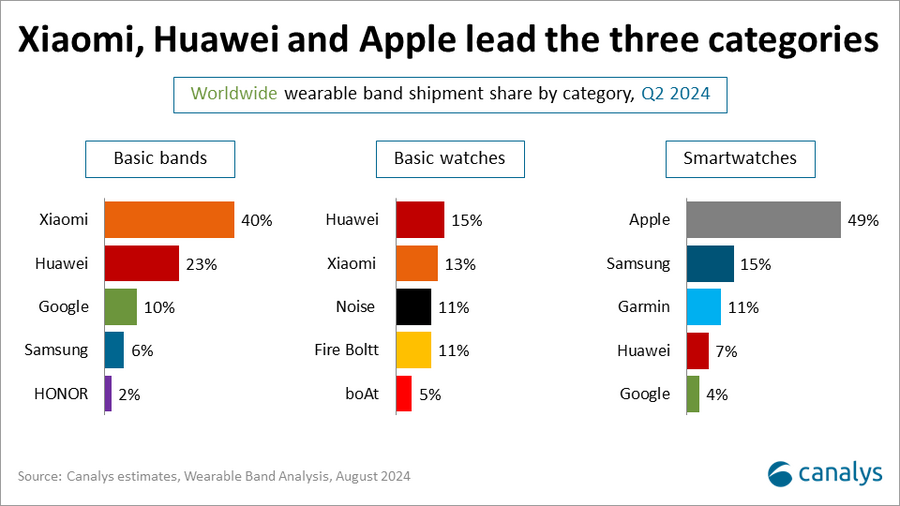
\includegraphics[width=1.0\linewidth]{./images/wearable_brand_diffusion.png}
    \caption[Wearable diffusion by major brands.]{Wearable diffusion by major brands \protect\cite{WearableDevicesBrandDiffusion}.}
    \label{fig:brandDiffusion}
\end{figure*}
\FloatBarrier
